\documentclass{article}
\setlength{\parskip}{5pt} % esp. entre parrafos
\setlength{\parindent}{0pt} % esp. al inicio de un parrafo
\usepackage{amsmath} % mates
\usepackage[sort&compress,numbers]{natbib} % referencias
\usepackage{url} % que las URLs se vean lindos
\usepackage[top=25mm,left=20mm,right=20mm,bottom=25mm]{geometry} % margenes
\usepackage{hyperref} % ligas de URLs
\usepackage{graphicx} % poner figuras
\usepackage[spanish]{babel} % otros idiomas
\usepackage[utf8]{inputenc} % alparecer son los acentos
\documentclass[12pt,letterpaper]{article}
\usepackage[utf8]{inputenc}
\usepackage{tikz}
\usetikzlibrary{trees}
\usepackage[spanish, es-nodecimaldot]{babel}
\usepackage{color}
\usepackage{algorithm}
\usepackage[noend]{algpseudocode}
\renewcommand{\algorithmicrequire}{\textbf{Entrada:}}
\renewcommand{\algorithmicensure}{\textbf{Salida:}}
\usepackage{subcaption}
\usepackage{amsfonts}
\usepackage{hyperref}
 \hypersetup{
     colorlinks=true,
     linkcolor=blue,
     filecolor=blue,
     citecolor = blue,      
     urlcolor=cyan,
     }
\usepackage{amssymb}
\usepackage{listings}
\usepackage{color}
\author{I E G} % author
\title{Práctica 4 : diagramas de Voronoi} % titulo
\date{\today}

\begin{document} % inicia contenido

\maketitle % cabecera

\begin{abstract} % resumen

Examina el efecto del número de semillas $k$, manteniendo \cite{elis4} constante el tamaño de la zona $n$, en la penetración de las grietas que se forman en términos de la mayor distancia Manhattan entre la grieta y el exterior de la pieza, visualizando los resultados con diagramas caja-bijote o similar sobre las réplicas y aplicando métodos estadísticos para establecer el efecto tiene, si es que tenga, $k$ en ello.



\begin{figure} [h!]% figura
    \centering
    \includegraphics[width=70mm]{Figura1.png} % archivo
    \caption{Generación de semillas.}
    \label{fig1}
\end{figure}

\end{abstract}


\section{Desarrollo}

Para efectos de esta práctica se utiliza Python versión 3.9.6, primeramente se utiliza el código previamente reportado \cite{elis4} donde se colocaran las semillas, la zona empleada es constante de $n$=100 posteriormente se generan las semillas en la zona creada variando \cite{cae4} la cantidad de 40, 90, 180; una vez generada la zona se propaga la grieta y se calcula la distancia manhattan, final mente se genera un grafico de las distancias manhattan de las grietas en función de las semillas de la zona de distribución. 

\section{Experimento}
En la figura \ref{fig1} se observa un ejemplo de las celdas de Voronoi generadas en una zona de distribución de 100×100 para 90 semillas y en la figura \ref{fig2} se muestra las celdas generadas con su respectiva grieta. En la figura \ref{fig3} se muestrea la gráfica caja-bigote para representar los datos del desarrollo.

\begin{figure} [h!]% figura
    \centering
    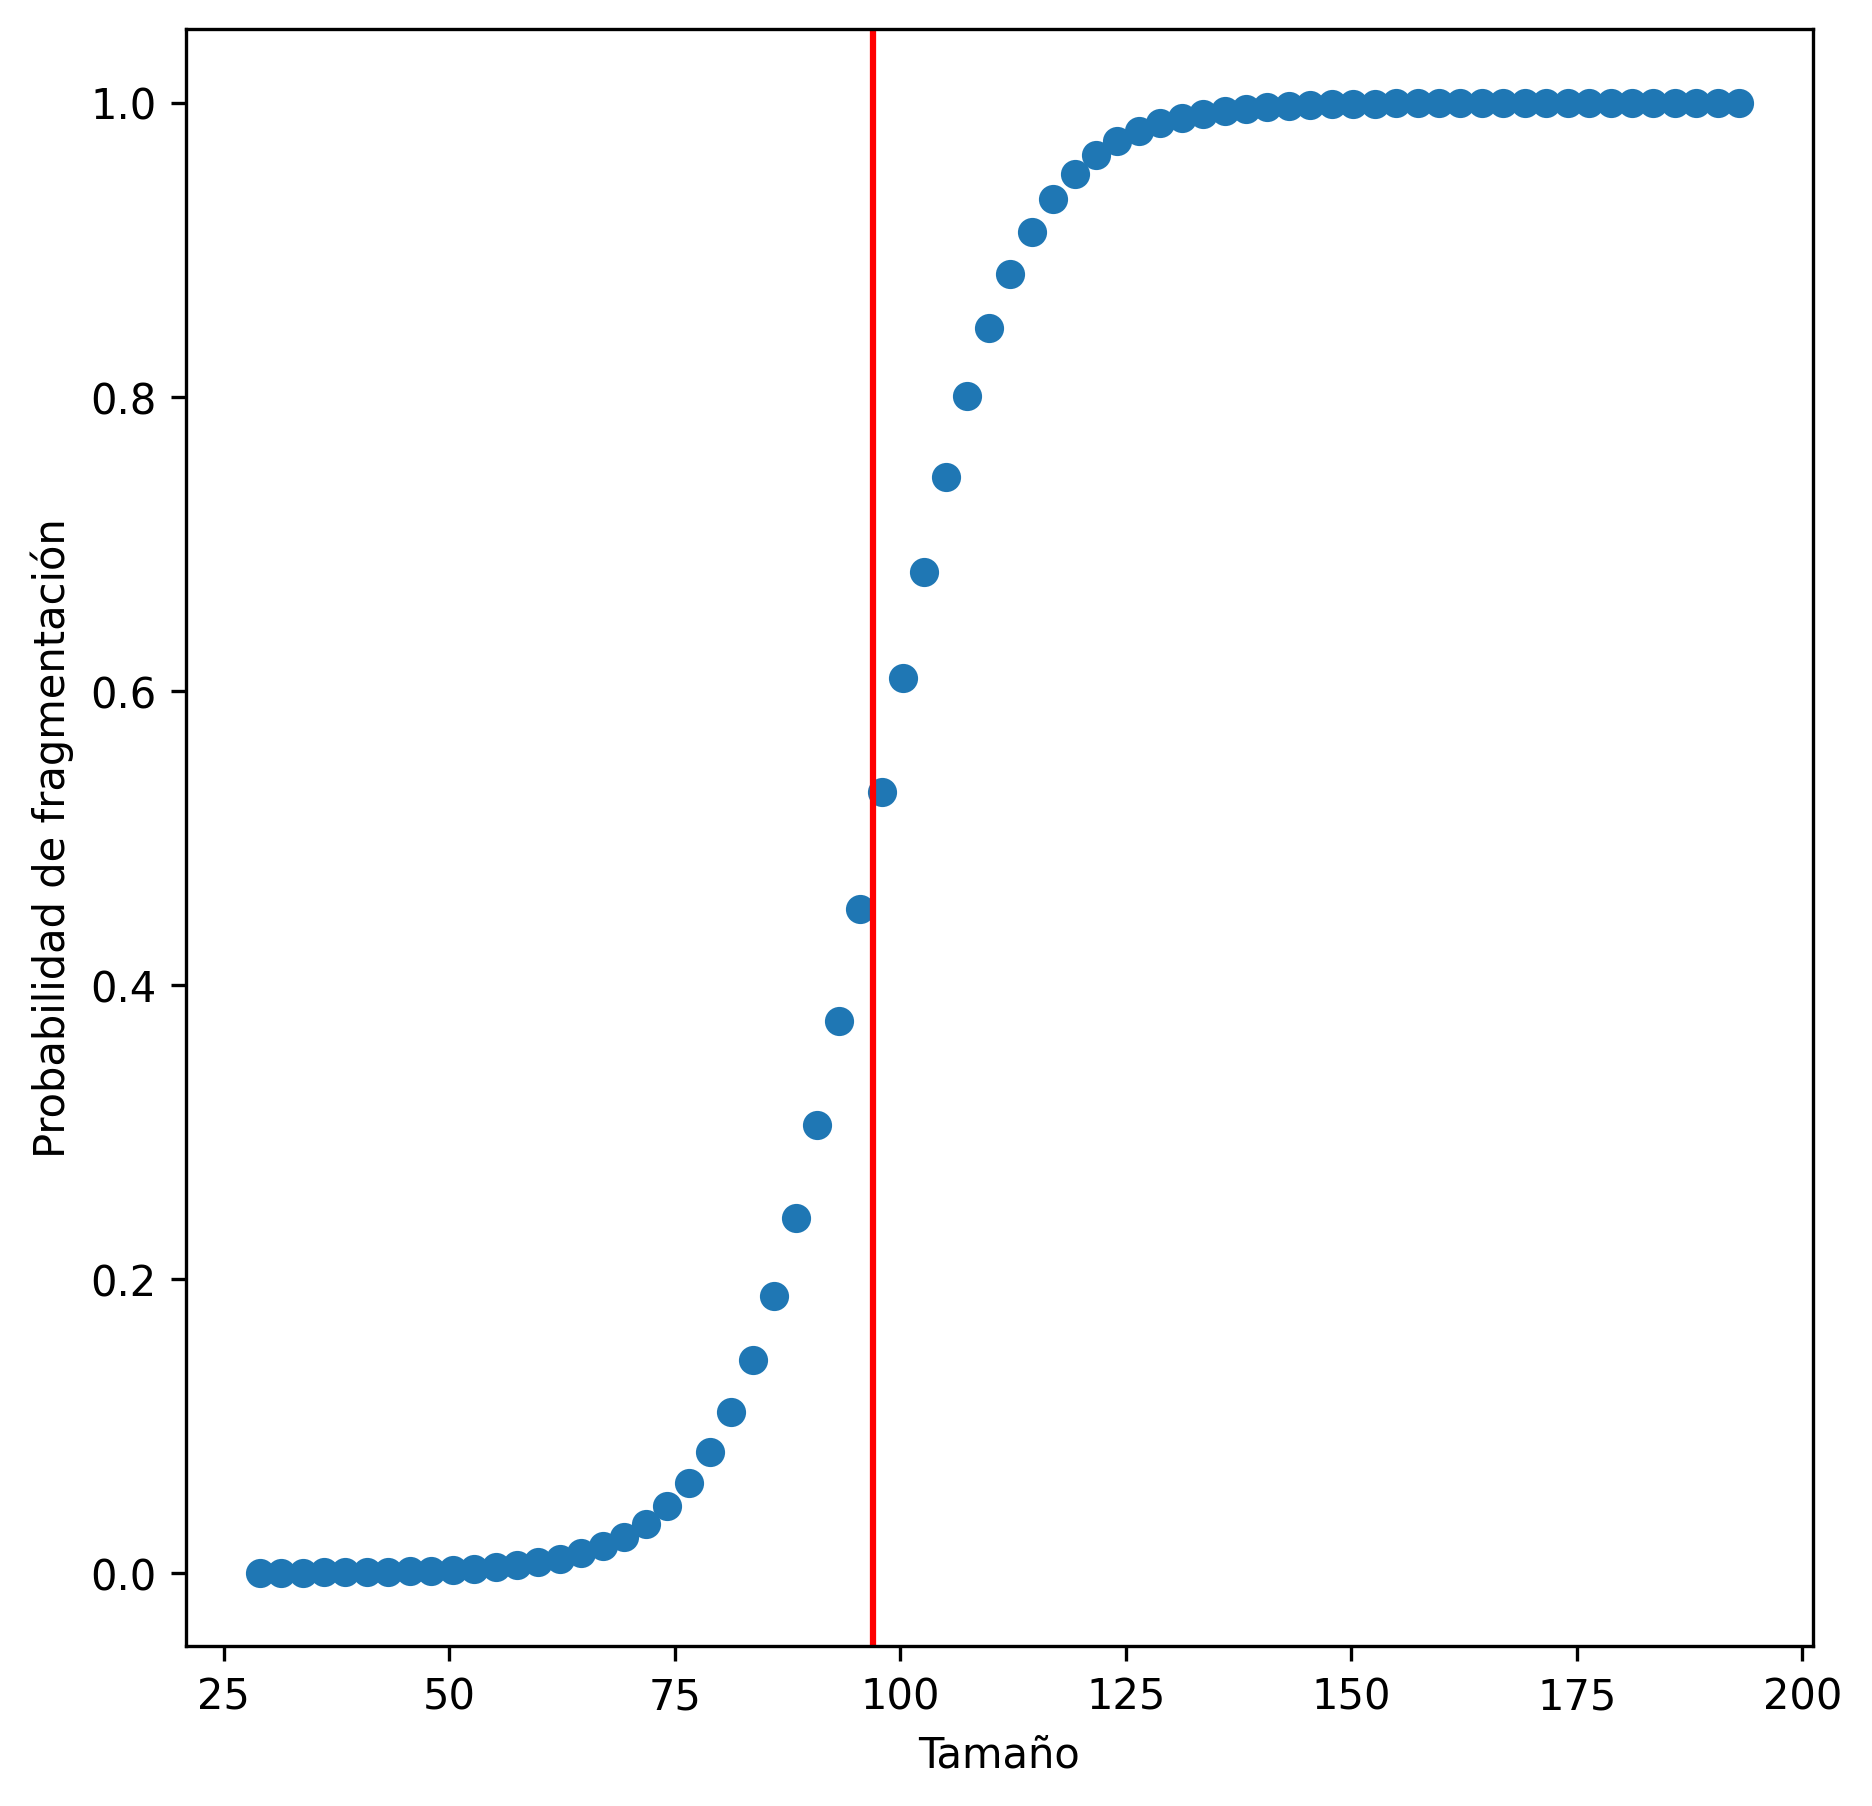
\includegraphics[width=100mm]{fig2.png} % archivo
    \caption{Celdas con grieta formada.}
    \label{fig2}
\end{figure}

\begin{figure} [h!]% figura
    \centering
    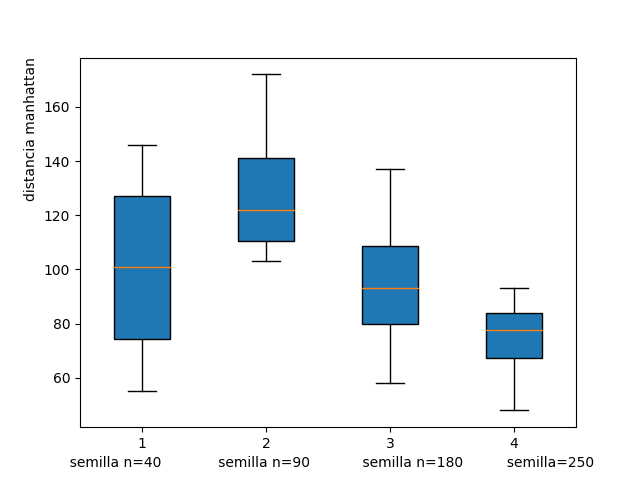
\includegraphics[width=100mm]{p4.png} % archivo
    \caption{Grafico caja-bigote.}
    \label{fig3}
\end{figure}
 

\section{Conclusiones} 

La distancia manhattan máxima de las grietas propagadas tiende a ser menor en tamaños de zona al aumentar la cantidad de semillas.




\bibliography{bib}
\bibliographystyle{plainnat}

\end{document}